\documentclass[9pt,pdftex]{beamer}
\setbeamertemplate{section in toc}[sections numbered]
\setbeamertemplate{subsection in toc}%
{\leavevmode\leftskip=3em\rlap{\hskip-2em\inserttocsectionnumber.\inserttocsubsectionnumber}\inserttocsubsection\par}
% use git: import repository as new project in eclipse: http://www.eclipse.org/forums/index.php/t/226301/
\usepackage[utf8]{inputenc}
\usepackage[english]{babel}
\usepackage{amsfonts, amsmath, amssymb}
\usepackage[bf,small, format=plain]{caption}
\usepackage{color}

%\usepackage[usenames,dvipsnames]{xcolor}
\usepackage{graphicx}
\usepackage{tikz,tikzscale,pgfplots,grffile}
\usetikzlibrary{arrows,shapes,backgrounds}
\usetikzlibrary{plotmarks}
\usepackage{bbding}

\usepackage[clock]{ifsym}

\usepackage{pgfplots}
\usepackage{grffile}
\pgfplotsset{compat=newest}

%\author{}
%\title{}
%\setbeamercovered{transparent} 
%\setbeamertemplate{navigation symbols}{} 
%\logo{} 
%\institute{} 
%\date{} 
%\subject{} 

\pgfdeclarelayer{bg}
\pgfsetlayers{bg,main}

\usepackage{listings}
\lstset{language=C++,
				tabsize=8,
				showtabs=true,
                basicstyle=\ttfamily,
                keywordstyle=\color{blue}\ttfamily,
                stringstyle=\color{red}\ttfamily,
                commentstyle=\color{green}\ttfamily,
                morecomment=[l][\color{magenta}]{\#}
}
\usepackage{mdframed}
\usepackage{multicol}
\usepackage{tcolorbox}
%\usepackage{multirow}
% \usepackage{paralist}
%\usepackage[colorinlistoftodos]{todonotes}
%\usepackage{biblatex}
%usepackage[nolist,nohyperlinks]{acronym}
%\usepackage{amstext}
%\usepackage{hyperref} 
%\usepackage{comment}
%\usepackage{subcaption}
%\renewcommand*{\figureautorefname}{fig.}
%\renewcommand*{\equationautorefname}{eq.}
\usepackage{bm}
\usepackage{comment}
%\usepackage{beamerthemeshadow}
%\usepackage{tikz}
%\usepackage{pgfplots}
%\usepackage{ulem}
%\usepackage[lofdepth,lotdepth]{subfig}
%\newenvironment{figure*}%
%{\begin{figure}}
%{\end{figure}}
%\usepackage[style=mla,babel=hyphen,backend=biber]{biblatex}
% CSE-Beamer-Styles:
\usepackage[course]{beamertheme_sccstalk}
%\usepackage[lecture]{beamertheme_sccstalk}
\usepackage{beamercolorscheme_sccs}
\usepackage{beamerfontthemestructurebold}
\setcounter{tocdepth}{3} 
%colored blocks, example \begin{variableblock}{Title}{bg=blue,fg=white}{bg=white,fg=black}
\newenvironment{variableblock}[4]{%
\setbeamercolor{block title}{#2}
\setbeamercolor{block body}{#3}
\begin{block}{#1}\begin{mdframed}{#4}\end{mdframed}\end{block}}


%some useful commands
%\newcommand{\der}[2]{\frac{\text{d}#1}{\text{d}#2}}
\title{Assignment 2: Parallel Debugging with TotalView}
\subtitle{Programming of Super Computers}
\author[Friedrich Menhorn, Benjamin Rüth, Erik Wannerberg] {Friedrich Menhorn, Benjamin Rüth, Erik Wannerberg \\ Team 12} %[displayed in footer]{displayed on title page}
\date{\today}
\institute{Technische Universität München}
\newtheorem*{rem}{Remark}


\begin{document}
\frame{\maketitle}

\section{Introduction}
\subsection{Contents}
\begin{frame}{Contents}
\tableofcontents
\end{frame}

\section{Task 3}
\subsection{Race Condition}
\begin{frame}{Race Condition}
\framesubtitle{Definition}
\begin{itemize}
\item From: \url{stackoverflow.com/questions/34510/what-is-a-race-condition}
\item[] "A race condition occurs when two or more threads can access shared data and they try to change it at the same time. Because the thread scheduling algorithm can swap between threads at any time, you don't know the order in which the threads will attempt to access the shared data. Therefore, the result of the change in data is dependent on the thread scheduling algorithm, i.e. both threads are "racing" to access/change the data."
\end{itemize}
\end{frame}

\begin{frame}[fragile]{Race Condition}
\framesubtitle{Test Code}
%\begin{itemize}
In \textbf{RaceCondition.cpp}
\scriptsize{
\begin{lstlisting} 
#include <iostream>
#include <omp.h>
int main(){
    int write,read;
    #pragma omp parallel shared(write) private(read)
    {
        write = omp_get_thread_num();
        if(omp_get_thread_num()==3){
            std::cout << "Thread: " << omp_get_thread_num() << 
            " Write: " << write << std::endl;
        }
        read = write;
        if(omp_get_thread_num()==3){
            std::cout << "Thread: " << omp_get_thread_num() << 
            " Read: " << read << std::endl;
        }
    }
    return 0;
}
\end{lstlisting}
}
%\end{itemize}
%\begin{mdframed}
Different outputs due to undefined order of access:\\
\begin{minipage}[t]{0.33\textwidth}
Output 1:
\scriptsize{
\begin{lstlisting}
$ ./RaceCondition 
Thread: 3 Write: 3
Thread: 3 Read: 3
\end{lstlisting}
}
\end{minipage}
%\hspace{1.3cm}
\begin{minipage}[t]{0.33\textwidth}
Output 2:
\scriptsize{
\begin{lstlisting}
$ ./RaceCondition 
Thread: 3 Write: 1
Thread: 3 Read: 1
\end{lstlisting}
}
\end{minipage}
\begin{minipage}[t]{0.33\textwidth}
Output 3:
\scriptsize{
\begin{lstlisting}
$ ./RaceCondition 
Thread: 3 Write: 3
Thread: 3 Read: 0
\end{lstlisting}
}
\end{minipage}
%\end{mdframed}
\end{frame}

\subsection{Deadlock}
\begin{frame}{Deadlock}
\framesubtitle{Definition}
\begin{itemize}
\item From: \url{https://en.wikipedia.org/wiki/Deadlock}
\item[] "In concurrent programming, a deadlock is a situation in which two or more competing actions are each waiting for the other to finish, and thus neither ever does."
\end{itemize}
\begin{figure}
\centering
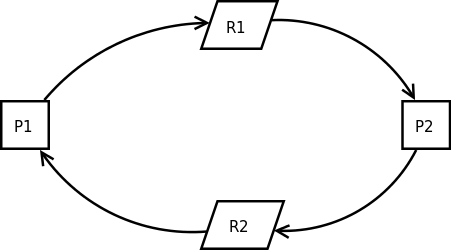
\includegraphics[scale=0.35]{img/Deadlock.png}
\end{figure}
\end{frame}

\subsection{Heisenbug}
\begin{frame}{Heisenbug}
\framesubtitle{Definition}
\begin{itemize}
\item From: \url{http://www.webopedia.com/TERM/H/heisenbug.html}
\item[] "In computer programming, heisenbug is a classification of an unusual software bug that disappears or alters its behavior when an attempt to isolate it is made.[...]"
\item From: \url{https://en.wikipedia.org/wiki/Heisenbug}
\item[] "One common example of a heisenbug is a bug that appears when the program is compiled with an optimizing compiler, but not when the same program is compiled without optimization.[...]"
\end{itemize}
\end{frame}

\subsection{Floating-point arithmetic challenges}
\subsubsection{Floating point comparison}
\begin{frame}[fragile]{Floating point comparison}
\framesubtitle{Test Code}
\begin{itemize}
\item[] In \textbf{FPComparison.cpp}
\scriptsize{
\begin{lstlisting} 
#include <iostream>
int main(){
    float a = 0.0;
    float b = 0.0;
    b = b - 0.1;
    b = b + 0.1;
    std::cout << "a: " << a << " b: " << b << std::endl;
    std::cout << "Comparison: " << (a==b) << std::endl;
    return 0;
}
\end{lstlisting}
}
\item[] \textbf{Output:}
\begin{lstlisting} 
$ ./FPComparison
a: 0 b: -1.49012e-09
Comparison: 0
\end{lstlisting}
\end{itemize}
\end{frame}

\subsubsection{Zero and signed zero}
\begin{frame}[fragile]{Zero and signed zero}
\framesubtitle{Definition}
\begin{itemize}
\item From: \url{http://www.johndcook.com/blog/2010/06/15/why-computers-have-signed-zero/}
\item[] "[...] computers have two versions of 0: positive zero and negative zero. Most of the time the distinction between +0 and -0 doesn’t matter, but once in a while signed versions of zero come in handy. [...]"
\item +0 and -0 to distinguish between the direction of underflowing to zero
\item[] "[...] The IEEE floating point standard says 1/+0 should be +infinity and 1/-0 should be -infinity.[...]"
\end{itemize}
\begin{mdframed}
\begin{minipage}[h]{0.4\textwidth}
Test Code:
\scriptsize{
\begin{lstlisting}
int main()
{
    double x = 1e-200;
    double y = 1e-200 * x;
    printf("Reciprocal of +0: %gn", 1/y);
    y = -1e-200*x;
    printf("Reciprocal of -0: %gn", 1/y);
}
\end{lstlisting}
}
\end{minipage}
\hspace{1.3cm}
\begin{minipage}[b]{0.4\textwidth}
Output:
\begin{lstlisting}
Reciprocal of +0: inf
Reciprocal of -0: -inf
\end{lstlisting}
\end{minipage}
\end{mdframed}
\end{frame}

\subsubsection{(Catastrophic) Cancellation}
\begin{frame}[fragile]{(Catastrophic) Cancellation}
\framesubtitle{Test Code}
\begin{itemize}
\item From \url{docs.oracle.com/cd/E19957-01/806-3568/ncg_goldberg.html}
\item Calculate $b^2-4ac$ in $x_{1/2}=\frac{-b \pm \sqrt{b^2-4ac}}{2a}$
\item With floating point precision (here $\approx_{fp}$) to \textbf{first digit!}
\item Example:
	\begin{itemize}
	\item Values: $b = 3.34; a = 1.22; c = 2.28$
	\item In one step: $b^2-4ac = \textcolor{red}{0.0292} \approx_{fp} \textcolor{blue}{0.0}$
	\item In single steps: 
				\begin{equation}
				\begin{split}
				&y  := b^2 = 11.1556 \approx_{fp} 11.2  \\
				&z := 4*a*c = 11.1264 \approx_{fp} 11.1 \\
				&y - z = 11.2-11.1 = \textcolor{green}{0.1}
				\end{split}
				\end{equation}
	\item Error:
				\begin{equation}
				\begin{split}
				&\text{One step: \quad } |\textcolor{red}{0.0292}- \textcolor{blue}{0.0}| = 0.0292 \\
				&\text{Single steps: } |\textcolor{red}{0.0292}-\textcolor{green}{0.1}| = 0.0708
				\end{split}
				\end{equation}
	\end{itemize}

\end{itemize}
\end{frame}

\subsubsection{Amplification and error propogation}
\begin{frame}[fragile]{Amplification and error propogation}
\framesubtitle{Test Code}
\begin{itemize}
\item[] In \textbf{ErrorPropagation.cpp}
\scriptsize{
\begin{lstlisting} 
#include <iostream> #include <iomanip> #include <math.h> 
int main(){
    float x = 0.0;
    float constant = 0.1;
    float exact;
    int curPow = 1;
    for(int i = 1; i <= 10000000; i++){
        x = x + constant;
        if( log10(i)==curPow){
            exact = i*constant;
            std::cout <<std::setprecision(8) << "# i: "<< i <<  " # x: " << x << 
            " Exact: " << exact << " Diff: " << exact-x << std::endl;
            curPow++;
        }	
    }
    return 0;
}
\end{lstlisting}
}
\item[] \textbf{Output:}
\begin{lstlisting}[language=java]
$ ./ErrorPropagation 
# i: 10 # x: 1.0000001 Exact: 1 Diff: -1.1920929e-07
# i: 100 # x: 10.000002 Exact: 10 Diff: -1.9073486e-06
...
# i: 100000 # x: 9998.5566 Exact: 10000 Diff: 1.4433594
# i: 1000000 # x: 100958.34 Exact: 100000 Diff: -958.34375
# i: 10000000 # x: 1087937 Exact: 1000000 Diff: -87937
\end{lstlisting}
\end{itemize}
\end{frame}

\begin{frame}[fragile]{Amplification and error propogation}
\framesubtitle{Definition}
\begin{itemize}
\item From: \url{http://floating-point-gui.de/errors/propagation/}
\item[] "While the errors in single floating-point numbers are very small, even simple calculations on them can contain pitfalls that increase the error in the result way beyond just having the individual errors “add up”.
\item[] In general:
\begin{itemize}
\item Multiplication and division are “safe” operations
\item Addition and subtraction are dangerous, because when numbers of different magnitudes are involved, digits of the smaller-magnitude number are lost.
\item This loss of digits can be inevitable and benign (when the lost digits also insignificant for the final result) or catastrophic (when the loss is magnified and distorts the result strongly).
\item The more calculations are done (especially when they form an iterative algorithm) the more important it is to consider this kind of problem.
\item $[...]$ "
\end{itemize}
\end{itemize}
\end{frame}

\subsection{Error exclusiveness to parallel programming}
\begin{frame}{Error exclusiveness to parallel programming}
Notation: 
\begin{itemize}
\item[\textcolor{green}{\checkmark}]: Problem does arise in this field 
\item[\textcolor{red}{\XSolidBrush}]: Problem does not arise in this field 
\end{itemize}
\begin{center}
  \begin{tabular}{ l || c | r }
    \hline
      & Sequential & Parallel \\ \hline
    FP arithmetic & \textcolor{green}{\checkmark} & \textcolor{green}{\checkmark} \\ \hline
    Heisenbug & \textcolor{green}{\checkmark} & \textcolor{green}{\checkmark} \\ \hline
    Race Condition & \textcolor{red}{\XSolidBrush} & \textcolor{green}{\checkmark} \\ \hline
    Deadlock & \textcolor{red}{\XSolidBrush} & \textcolor{green}{\checkmark} \\
    \hline
  \end{tabular}
\end{center}
\end{frame}

\section{Task 4}
\begin{frame}{Task 4}
\tableofcontents[
  currentsection,
  sectionstyle=show/hide,
  subsectionstyle=show/show/hide
]
\end{frame}
\subsection{TotalView GUI}
\subsubsection{Session manager}
\begin{frame}dummy\end{frame}
\subsubsection{Root window}
\begin{frame}dummy\end{frame}
\subsubsection{Process window}
\begin{frame}dummy\end{frame}
\subsubsection{Variable window}
\begin{frame}dummy\end{frame}
\subsection{TotalView Basic Operations}
\subsubsection{Control execution}
\begin{frame}dummy\end{frame}
\subsubsection{Setting breakpoints}
\begin{frame}dummy\end{frame}
\subsubsection{Diving into functions}
\begin{frame}dummy\end{frame}
\subsubsection{View memory}
\begin{frame}dummy\end{frame}

\section{Task 5}
\begin{frame}{Task 5}
\tableofcontents[
  currentsection,
  sectionstyle=show/hide,
  subsectionstyle=show/show/hide
]
\end{frame}
\subsection{OpenMP Fork-Join Model}
\begin{frame}dummy\end{frame}
\subsection{TotalView and OpenMP}
\begin{frame}dummy\end{frame}

\section{Task 6}
\begin{frame}{Task 6}
\tableofcontents[
  currentsection,
  sectionstyle=show/hide,
  subsectionstyle=show/show/hide
]
\end{frame}
\subsection{TotalView and MPI}
\begin{frame}dummy\end{frame}
\subsection{Visualize arrays in TotalView}
\begin{frame}dummy\end{frame}

\end{document}
